\documentclass[twoside]{book}

% Packages required by doxygen
\usepackage{fixltx2e}
\usepackage{calc}
\usepackage{doxygen}
\usepackage[export]{adjustbox} % also loads graphicx
\usepackage{graphicx}
\usepackage[utf8]{inputenc}
\usepackage{makeidx}
\usepackage{multicol}
\usepackage{multirow}
\PassOptionsToPackage{warn}{textcomp}
\usepackage{textcomp}
\usepackage[nointegrals]{wasysym}
\usepackage[table]{xcolor}

% Font selection
\usepackage[T1]{fontenc}
\usepackage[scaled=.90]{helvet}
\usepackage{courier}
\usepackage{amssymb}
\usepackage{sectsty}
\renewcommand{\familydefault}{\sfdefault}
\allsectionsfont{%
  \fontseries{bc}\selectfont%
  \color{darkgray}%
}
\renewcommand{\DoxyLabelFont}{%
  \fontseries{bc}\selectfont%
  \color{darkgray}%
}
\newcommand{\+}{\discretionary{\mbox{\scriptsize$\hookleftarrow$}}{}{}}

% Page & text layout
\usepackage{geometry}
\geometry{%
  a4paper,%
  top=2.5cm,%
  bottom=2.5cm,%
  left=2.5cm,%
  right=2.5cm%
}
\tolerance=750
\hfuzz=15pt
\hbadness=750
\setlength{\emergencystretch}{15pt}
\setlength{\parindent}{0cm}
\setlength{\parskip}{3ex plus 2ex minus 2ex}
\makeatletter
\renewcommand{\paragraph}{%
  \@startsection{paragraph}{4}{0ex}{-1.0ex}{1.0ex}{%
    \normalfont\normalsize\bfseries\SS@parafont%
  }%
}
\renewcommand{\subparagraph}{%
  \@startsection{subparagraph}{5}{0ex}{-1.0ex}{1.0ex}{%
    \normalfont\normalsize\bfseries\SS@subparafont%
  }%
}
\makeatother

% Headers & footers
\usepackage{fancyhdr}
\pagestyle{fancyplain}
\fancyhead[LE]{\fancyplain{}{\bfseries\thepage}}
\fancyhead[CE]{\fancyplain{}{}}
\fancyhead[RE]{\fancyplain{}{\bfseries\leftmark}}
\fancyhead[LO]{\fancyplain{}{\bfseries\rightmark}}
\fancyhead[CO]{\fancyplain{}{}}
\fancyhead[RO]{\fancyplain{}{\bfseries\thepage}}
\fancyfoot[LE]{\fancyplain{}{}}
\fancyfoot[CE]{\fancyplain{}{}}
\fancyfoot[RE]{\fancyplain{}{\bfseries\scriptsize Generated by Doxygen }}
\fancyfoot[LO]{\fancyplain{}{\bfseries\scriptsize Generated by Doxygen }}
\fancyfoot[CO]{\fancyplain{}{}}
\fancyfoot[RO]{\fancyplain{}{}}
\renewcommand{\footrulewidth}{0.4pt}
\renewcommand{\chaptermark}[1]{%
  \markboth{#1}{}%
}
\renewcommand{\sectionmark}[1]{%
  \markright{\thesection\ #1}%
}

% Indices & bibliography
\usepackage{natbib}
\usepackage[titles]{tocloft}
\setcounter{tocdepth}{3}
\setcounter{secnumdepth}{5}
\makeindex

% Hyperlinks (required, but should be loaded last)
\usepackage{ifpdf}
\ifpdf
  \usepackage[pdftex,pagebackref=true]{hyperref}
\else
  \usepackage[ps2pdf,pagebackref=true]{hyperref}
\fi
\hypersetup{%
  colorlinks=true,%
  linkcolor=blue,%
  citecolor=blue,%
  unicode%
}

% Custom commands
\newcommand{\clearemptydoublepage}{%
  \newpage{\pagestyle{empty}\cleardoublepage}%
}

\usepackage{caption}
\captionsetup{labelsep=space,justification=centering,font={bf},singlelinecheck=off,skip=4pt,position=top}

%===== C O N T E N T S =====

\begin{document}

% Titlepage & ToC
\hypersetup{pageanchor=false,
             bookmarksnumbered=true,
             pdfencoding=unicode
            }
\pagenumbering{roman}
\begin{titlepage}
\vspace*{7cm}
\begin{center}%
{\Large My Project }\\
\vspace*{1cm}
{\large Generated by Doxygen 1.8.11}\\
\end{center}
\end{titlepage}
\clearemptydoublepage
\tableofcontents
\clearemptydoublepage
\pagenumbering{arabic}
\hypersetup{pageanchor=true}

%--- Begin generated contents ---
\chapter{Hierarchical Index}
\section{Class Hierarchy}
This inheritance list is sorted roughly, but not completely, alphabetically\+:\begin{DoxyCompactList}
\item exception\begin{DoxyCompactList}
\item \contentsline{section}{Process\+Exception}{\pageref{class_process_exception}}{}
\begin{DoxyCompactList}
\item \contentsline{section}{Config\+Exception}{\pageref{class_config_exception}}{}
\item \contentsline{section}{Invalid\+Key\+Exception}{\pageref{class_invalid_key_exception}}{}
\item \contentsline{section}{Multiple\+Key\+Exception}{\pageref{class_multiple_key_exception}}{}
\item \contentsline{section}{Plugin\+Init\+Exception}{\pageref{class_plugin_init_exception}}{}
\item \contentsline{section}{Plugin\+Load\+Exception}{\pageref{class_plugin_load_exception}}{}
\end{DoxyCompactList}
\end{DoxyCompactList}
\item Q\+Object\begin{DoxyCompactList}
\item \contentsline{section}{Abstract\+Process}{\pageref{class_abstract_process}}{}
\end{DoxyCompactList}
\end{DoxyCompactList}

\chapter{Class Index}
\section{Class List}
Here are the classes, structs, unions and interfaces with brief descriptions\+:\begin{DoxyCompactList}
\item\contentsline{section}{\hyperlink{class_abstract_process}{Abstract\+Process} \\*The \hyperlink{class_abstract_process}{Abstract\+Process} class  Класс процеса, расширяемого плагинами }{\pageref{class_abstract_process}}{}
\item\contentsline{section}{\hyperlink{class_config_exception}{Config\+Exception} }{\pageref{class_config_exception}}{}
\item\contentsline{section}{\hyperlink{class_invalid_key_exception}{Invalid\+Key\+Exception} }{\pageref{class_invalid_key_exception}}{}
\item\contentsline{section}{\hyperlink{class_multiple_key_exception}{Multiple\+Key\+Exception} }{\pageref{class_multiple_key_exception}}{}
\item\contentsline{section}{\hyperlink{class_plugin_init_exception}{Plugin\+Init\+Exception} }{\pageref{class_plugin_init_exception}}{}
\item\contentsline{section}{\hyperlink{class_plugin_load_exception}{Plugin\+Load\+Exception} }{\pageref{class_plugin_load_exception}}{}
\item\contentsline{section}{\hyperlink{class_process_exception}{Process\+Exception} }{\pageref{class_process_exception}}{}
\end{DoxyCompactList}

\chapter{File Index}
\section{File List}
Here is a list of all files with brief descriptions\+:\begin{DoxyCompactList}
\item\contentsline{section}{src/abstractprocess/\hyperlink{abstractprocess_8cpp}{abstractprocess.\+cpp} }{\pageref{abstractprocess_8cpp}}{}
\item\contentsline{section}{src/abstractprocess/\hyperlink{abstractprocess_8h}{abstractprocess.\+h} }{\pageref{abstractprocess_8h}}{}
\item\contentsline{section}{src/abstractprocess/\hyperlink{main_8cpp}{main.\+cpp} }{\pageref{main_8cpp}}{}
\item\contentsline{section}{src/abstractprocess/\hyperlink{processexceptions_8h}{processexceptions.\+h} }{\pageref{processexceptions_8h}}{}
\end{DoxyCompactList}

\chapter{Class Documentation}
\hypertarget{class_abstract_process}{}\section{Abstract\+Process Class Reference}
\label{class_abstract_process}\index{Abstract\+Process@{Abstract\+Process}}


The \hyperlink{class_abstract_process}{Abstract\+Process} class  Класс процеса, расширяемого плагинами  




{\ttfamily \#include $<$abstractprocess.\+h$>$}

Inheritance diagram for Abstract\+Process\+:\begin{figure}[H]
\begin{center}
\leavevmode
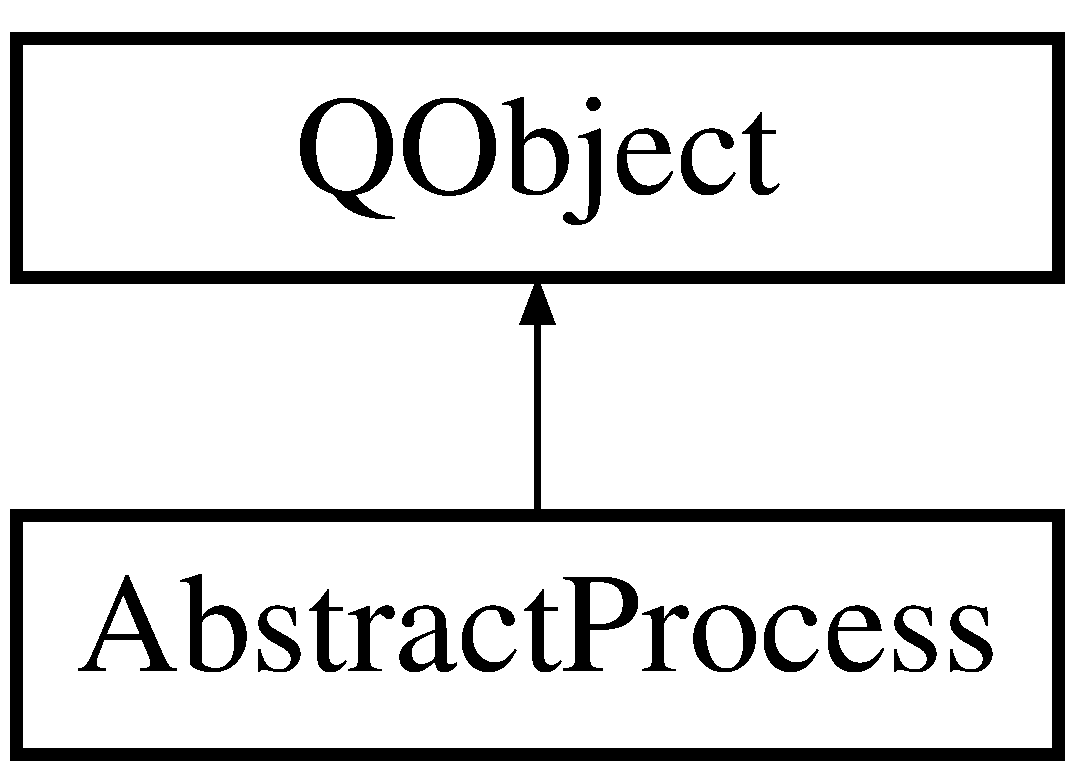
\includegraphics[height=2.000000cm]{class_abstract_process}
\end{center}
\end{figure}
\subsection*{Public Member Functions}
\begin{DoxyCompactItemize}
\item 
\hyperlink{class_abstract_process_a6e39ac735166365e2a844aff7c0bc6e4}{Abstract\+Process} (Q\+Map$<$ Q\+String, Q\+String $>$ \&arguments, Q\+Object $\ast$parent=0)  throw (std\+::invalid\+\_\+argument)
\item 
\hyperlink{class_abstract_process_a585a0cfa21de4b8dc84612424f83afd4}{$\sim$\+Abstract\+Process} ()
\item 
int \hyperlink{class_abstract_process_ad567aa24b1ea6121a29a01b14f5bcf86}{init} (int argc, char $\ast$argv\mbox{[}$\,$\mbox{]})  throw (\+Process\+Exception)
\begin{DoxyCompactList}\small\item\em process\+Config  Разбор файла конфигурации, создание плагинов, передача данных версий процесса и плагинов в ядро и настройка объектов межпроцессного взаимодействия, указанных в файле конфигурации \end{DoxyCompactList}\end{DoxyCompactItemize}
\subsection*{Static Public Member Functions}
\begin{DoxyCompactItemize}
\item 
static Q\+Hash$<$ Q\+String, Q\+String $>$ \hyperlink{class_abstract_process_abf4a14110a0255fbade7d7b89792abfe}{arguments\+Parse} (const char $\ast$keys, int argc, char $\ast$argv\mbox{[}$\,$\mbox{]})  throw (\+Invalid\+Key\+Exception,                                                                                                 Multiple\+Key\+Exception)
\begin{DoxyCompactList}\small\item\em arguments\+Parse -\/ разбор строки с аргументами процессов \end{DoxyCompactList}\end{DoxyCompactItemize}


\subsection{Detailed Description}
The \hyperlink{class_abstract_process}{Abstract\+Process} class  Класс процеса, расширяемого плагинами 

Definition at line 21 of file abstractprocess.\+h.



\subsection{Constructor \& Destructor Documentation}
\index{Abstract\+Process@{Abstract\+Process}!Abstract\+Process@{Abstract\+Process}}
\index{Abstract\+Process@{Abstract\+Process}!Abstract\+Process@{Abstract\+Process}}
\subsubsection[{\texorpdfstring{Abstract\+Process(\+Q\+Map$<$ Q\+String, Q\+String $>$ \&arguments, Q\+Object $\ast$parent=0)}{AbstractProcess(QMap< QString, QString > &arguments, QObject *parent=0)}}]{\setlength{\rightskip}{0pt plus 5cm}Abstract\+Process\+::\+Abstract\+Process (
\begin{DoxyParamCaption}
\item[{Q\+Map$<$ Q\+String, Q\+String $>$ \&}]{arguments, }
\item[{Q\+Object $\ast$}]{parent = {\ttfamily 0}}
\end{DoxyParamCaption}
) throw  std\+::invalid\+\_\+argument) \hspace{0.3cm}{\ttfamily [explicit]}}\hypertarget{class_abstract_process_a6e39ac735166365e2a844aff7c0bc6e4}{}\label{class_abstract_process_a6e39ac735166365e2a844aff7c0bc6e4}


Definition at line 11 of file abstractprocess.\+cpp.

\index{Abstract\+Process@{Abstract\+Process}!````~Abstract\+Process@{$\sim$\+Abstract\+Process}}
\index{````~Abstract\+Process@{$\sim$\+Abstract\+Process}!Abstract\+Process@{Abstract\+Process}}
\subsubsection[{\texorpdfstring{$\sim$\+Abstract\+Process()}{~AbstractProcess()}}]{\setlength{\rightskip}{0pt plus 5cm}Abstract\+Process\+::$\sim$\+Abstract\+Process (
\begin{DoxyParamCaption}
{}
\end{DoxyParamCaption}
)}\hypertarget{class_abstract_process_a585a0cfa21de4b8dc84612424f83afd4}{}\label{class_abstract_process_a585a0cfa21de4b8dc84612424f83afd4}


Definition at line 24 of file abstractprocess.\+cpp.



\subsection{Member Function Documentation}
\index{Abstract\+Process@{Abstract\+Process}!arguments\+Parse@{arguments\+Parse}}
\index{arguments\+Parse@{arguments\+Parse}!Abstract\+Process@{Abstract\+Process}}
\subsubsection[{\texorpdfstring{arguments\+Parse(const char $\ast$keys, int argc, char $\ast$argv[])}{argumentsParse(const char *keys, int argc, char *argv[])}}]{\setlength{\rightskip}{0pt plus 5cm}Q\+Hash$<$ Q\+String, Q\+String $>$ Abstract\+Process\+::arguments\+Parse (
\begin{DoxyParamCaption}
\item[{const char $\ast$}]{keys, }
\item[{int}]{argc, }
\item[{char $\ast$}]{argv\mbox{[}$\,$\mbox{]}}
\end{DoxyParamCaption}
) throw  {\bf Invalid\+Key\+Exception},                                                                                                                                                                                                {\bf Multiple\+Key\+Exception}) \hspace{0.3cm}{\ttfamily [static]}}\hypertarget{class_abstract_process_abf4a14110a0255fbade7d7b89792abfe}{}\label{class_abstract_process_abf4a14110a0255fbade7d7b89792abfe}


arguments\+Parse -\/ разбор строки с аргументами процессов 


\begin{DoxyParams}{Parameters}
{\em keys} & -\/ строка с ключами \\
\hline
{\em argc} & -\/ количество аргументов \\
\hline
{\em argv} & -\/ массив строк \\
\hline
\end{DoxyParams}
\begin{DoxyReturn}{Returns}
map с ключами и его значениями 
\end{DoxyReturn}


Definition at line 29 of file abstractprocess.\+cpp.

\index{Abstract\+Process@{Abstract\+Process}!init@{init}}
\index{init@{init}!Abstract\+Process@{Abstract\+Process}}
\subsubsection[{\texorpdfstring{init(int argc, char $\ast$argv[])}{init(int argc, char *argv[])}}]{\setlength{\rightskip}{0pt plus 5cm}int Abstract\+Process\+::init (
\begin{DoxyParamCaption}
\item[{int}]{argc, }
\item[{char $\ast$}]{argv\mbox{[}$\,$\mbox{]}}
\end{DoxyParamCaption}
) throw  {\bf Process\+Exception}) }\hypertarget{class_abstract_process_ad567aa24b1ea6121a29a01b14f5bcf86}{}\label{class_abstract_process_ad567aa24b1ea6121a29a01b14f5bcf86}


process\+Config  Разбор файла конфигурации, создание плагинов, передача данных версий процесса и плагинов в ядро и настройка объектов межпроцессного взаимодействия, указанных в файле конфигурации 



Definition at line 123 of file abstractprocess.\+cpp.



The documentation for this class was generated from the following files\+:\begin{DoxyCompactItemize}
\item 
src/abstractprocess/\hyperlink{abstractprocess_8h}{abstractprocess.\+h}\item 
src/abstractprocess/\hyperlink{abstractprocess_8cpp}{abstractprocess.\+cpp}\end{DoxyCompactItemize}

\hypertarget{class_config_exception}{}\section{Config\+Exception Class Reference}
\label{class_config_exception}\index{Config\+Exception@{Config\+Exception}}


{\ttfamily \#include $<$processexceptions.\+h$>$}

Inheritance diagram for Config\+Exception\+:\begin{figure}[H]
\begin{center}
\leavevmode
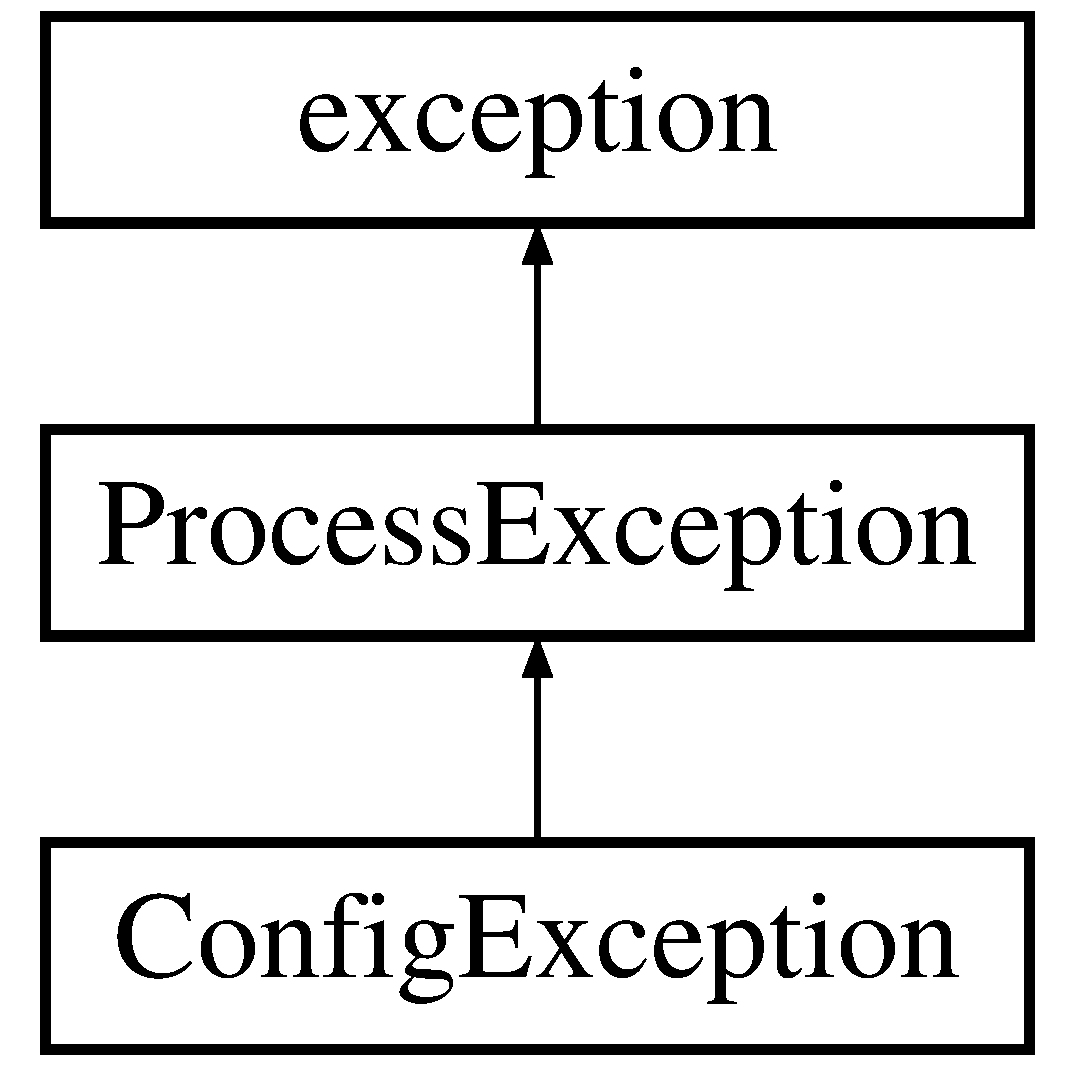
\includegraphics[height=3.000000cm]{class_config_exception}
\end{center}
\end{figure}
\subsection*{Public Member Functions}
\begin{DoxyCompactItemize}
\item 
\hyperlink{class_config_exception_ab0f298b4e0680c6704f6d9da2708b944}{Config\+Exception} (const std\+::string \&msg)
\item 
virtual \hyperlink{class_config_exception_ab70bb87e3f4e6d03d3080c114844c57a}{$\sim$\+Config\+Exception} () noexcept
\end{DoxyCompactItemize}


\subsection{Detailed Description}


Definition at line 43 of file processexceptions.\+h.



\subsection{Constructor \& Destructor Documentation}
\index{Config\+Exception@{Config\+Exception}!Config\+Exception@{Config\+Exception}}
\index{Config\+Exception@{Config\+Exception}!Config\+Exception@{Config\+Exception}}
\subsubsection[{\texorpdfstring{Config\+Exception(const std\+::string \&msg)}{ConfigException(const std::string &msg)}}]{\setlength{\rightskip}{0pt plus 5cm}Config\+Exception\+::\+Config\+Exception (
\begin{DoxyParamCaption}
\item[{const std\+::string \&}]{msg}
\end{DoxyParamCaption}
)\hspace{0.3cm}{\ttfamily [inline]}}\hypertarget{class_config_exception_ab0f298b4e0680c6704f6d9da2708b944}{}\label{class_config_exception_ab0f298b4e0680c6704f6d9da2708b944}


Definition at line 46 of file processexceptions.\+h.

\index{Config\+Exception@{Config\+Exception}!````~Config\+Exception@{$\sim$\+Config\+Exception}}
\index{````~Config\+Exception@{$\sim$\+Config\+Exception}!Config\+Exception@{Config\+Exception}}
\subsubsection[{\texorpdfstring{$\sim$\+Config\+Exception() noexcept}{~ConfigException() noexcept}}]{\setlength{\rightskip}{0pt plus 5cm}virtual Config\+Exception\+::$\sim$\+Config\+Exception (
\begin{DoxyParamCaption}
{}
\end{DoxyParamCaption}
)\hspace{0.3cm}{\ttfamily [inline]}, {\ttfamily [virtual]}, {\ttfamily [noexcept]}}\hypertarget{class_config_exception_ab70bb87e3f4e6d03d3080c114844c57a}{}\label{class_config_exception_ab70bb87e3f4e6d03d3080c114844c57a}


Definition at line 49 of file processexceptions.\+h.



The documentation for this class was generated from the following file\+:\begin{DoxyCompactItemize}
\item 
src/abstractprocess/\hyperlink{processexceptions_8h}{processexceptions.\+h}\end{DoxyCompactItemize}

\hypertarget{class_invalid_key_exception}{}\section{Invalid\+Key\+Exception Class Reference}
\label{class_invalid_key_exception}\index{Invalid\+Key\+Exception@{Invalid\+Key\+Exception}}


{\ttfamily \#include $<$processexceptions.\+h$>$}

Inheritance diagram for Invalid\+Key\+Exception\+:\begin{figure}[H]
\begin{center}
\leavevmode
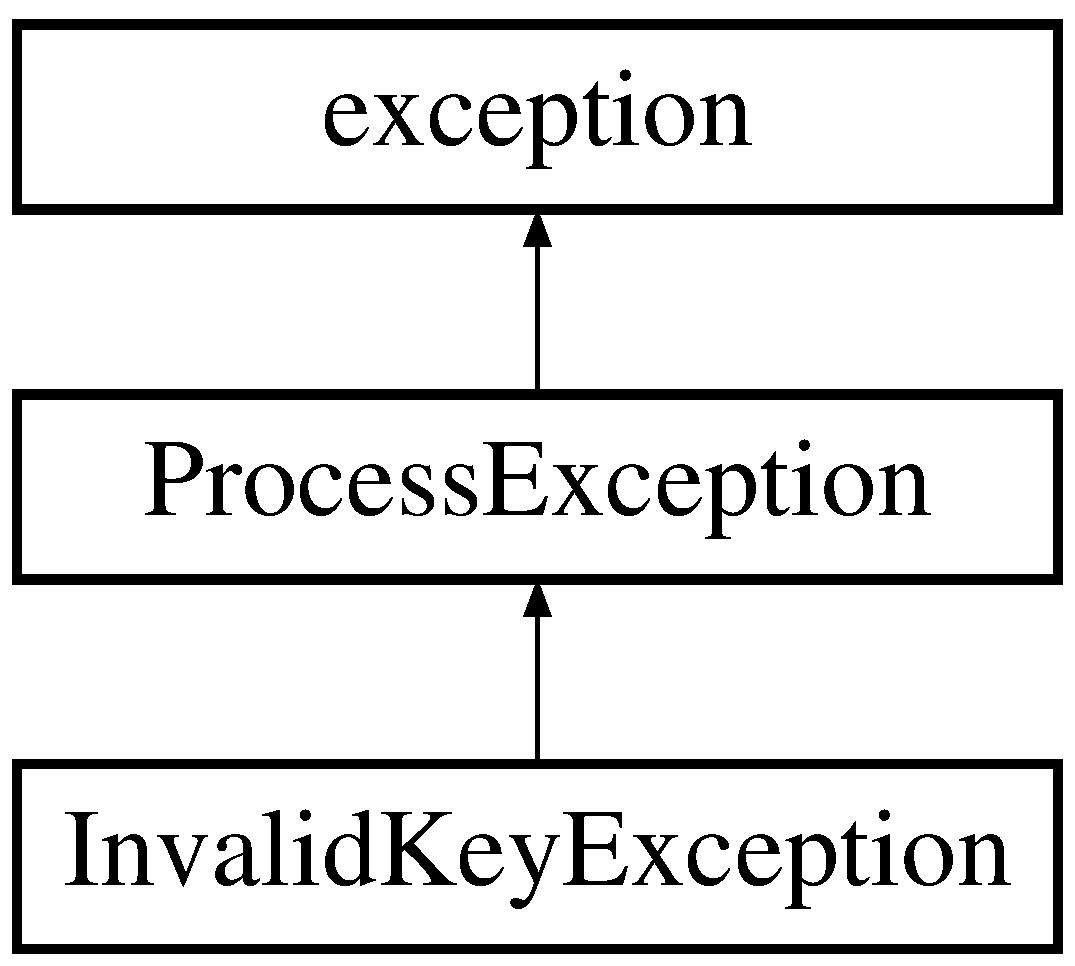
\includegraphics[height=3.000000cm]{class_invalid_key_exception}
\end{center}
\end{figure}
\subsection*{Public Member Functions}
\begin{DoxyCompactItemize}
\item 
\hyperlink{class_invalid_key_exception_a46442c3519b5707dddfb83f5dde943e0}{Invalid\+Key\+Exception} (const std\+::string \&msg)
\item 
virtual \hyperlink{class_invalid_key_exception_abfa7a065a197e4a85c1e5e862d282e5e}{$\sim$\+Invalid\+Key\+Exception} () noexcept
\end{DoxyCompactItemize}


\subsection{Detailed Description}


Definition at line 24 of file processexceptions.\+h.



\subsection{Constructor \& Destructor Documentation}
\index{Invalid\+Key\+Exception@{Invalid\+Key\+Exception}!Invalid\+Key\+Exception@{Invalid\+Key\+Exception}}
\index{Invalid\+Key\+Exception@{Invalid\+Key\+Exception}!Invalid\+Key\+Exception@{Invalid\+Key\+Exception}}
\subsubsection[{\texorpdfstring{Invalid\+Key\+Exception(const std\+::string \&msg)}{InvalidKeyException(const std::string &msg)}}]{\setlength{\rightskip}{0pt plus 5cm}Invalid\+Key\+Exception\+::\+Invalid\+Key\+Exception (
\begin{DoxyParamCaption}
\item[{const std\+::string \&}]{msg}
\end{DoxyParamCaption}
)\hspace{0.3cm}{\ttfamily [inline]}}\hypertarget{class_invalid_key_exception_a46442c3519b5707dddfb83f5dde943e0}{}\label{class_invalid_key_exception_a46442c3519b5707dddfb83f5dde943e0}


Definition at line 27 of file processexceptions.\+h.

\index{Invalid\+Key\+Exception@{Invalid\+Key\+Exception}!````~Invalid\+Key\+Exception@{$\sim$\+Invalid\+Key\+Exception}}
\index{````~Invalid\+Key\+Exception@{$\sim$\+Invalid\+Key\+Exception}!Invalid\+Key\+Exception@{Invalid\+Key\+Exception}}
\subsubsection[{\texorpdfstring{$\sim$\+Invalid\+Key\+Exception() noexcept}{~InvalidKeyException() noexcept}}]{\setlength{\rightskip}{0pt plus 5cm}virtual Invalid\+Key\+Exception\+::$\sim$\+Invalid\+Key\+Exception (
\begin{DoxyParamCaption}
{}
\end{DoxyParamCaption}
)\hspace{0.3cm}{\ttfamily [inline]}, {\ttfamily [virtual]}, {\ttfamily [noexcept]}}\hypertarget{class_invalid_key_exception_abfa7a065a197e4a85c1e5e862d282e5e}{}\label{class_invalid_key_exception_abfa7a065a197e4a85c1e5e862d282e5e}


Definition at line 30 of file processexceptions.\+h.



The documentation for this class was generated from the following file\+:\begin{DoxyCompactItemize}
\item 
src/abstractprocess/\hyperlink{processexceptions_8h}{processexceptions.\+h}\end{DoxyCompactItemize}

\hypertarget{class_multiple_key_exception}{}\section{Multiple\+Key\+Exception Class Reference}
\label{class_multiple_key_exception}\index{Multiple\+Key\+Exception@{Multiple\+Key\+Exception}}


{\ttfamily \#include $<$processexceptions.\+h$>$}

Inheritance diagram for Multiple\+Key\+Exception\+:\begin{figure}[H]
\begin{center}
\leavevmode
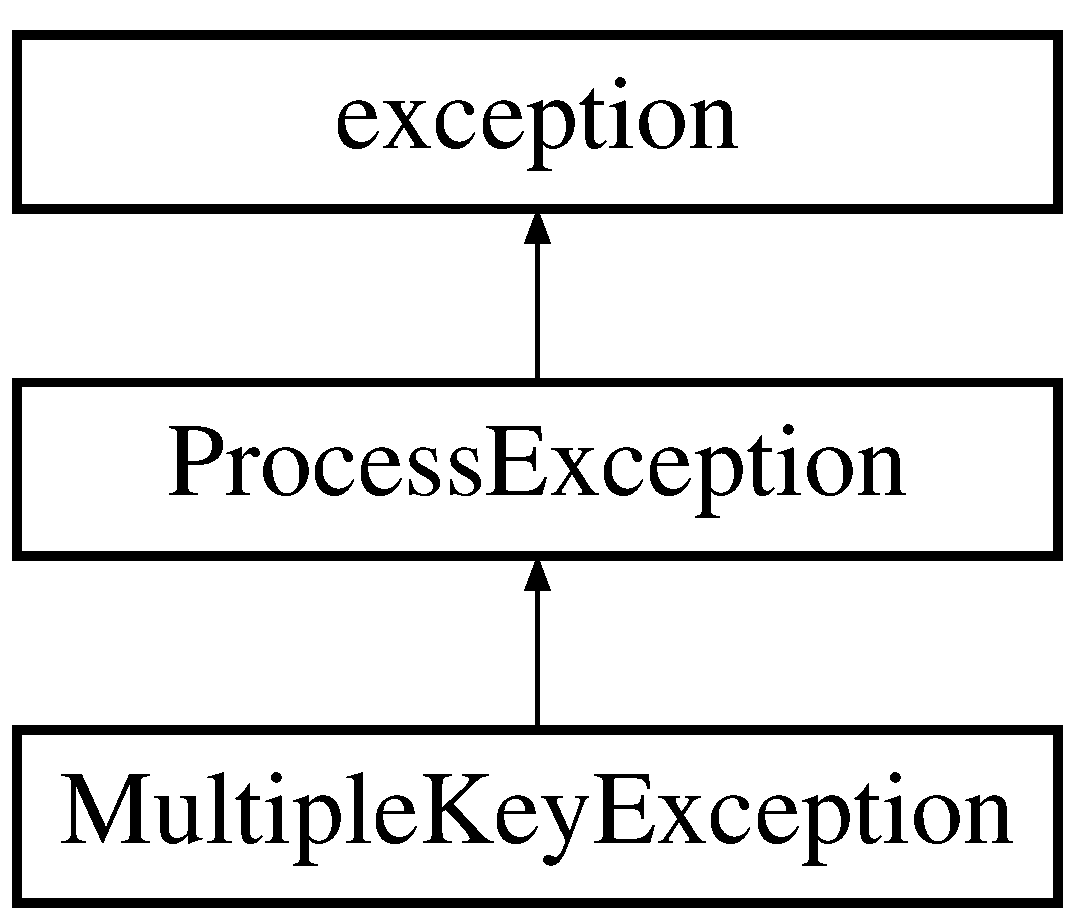
\includegraphics[height=3.000000cm]{class_multiple_key_exception}
\end{center}
\end{figure}
\subsection*{Public Member Functions}
\begin{DoxyCompactItemize}
\item 
\hyperlink{class_multiple_key_exception_adf1ee2101bd8ce66a80e48d5f49c86f9}{Multiple\+Key\+Exception} (const std\+::string \&msg)
\item 
virtual \hyperlink{class_multiple_key_exception_a0c1dfc4a0ddfc5d1c6618ae3f129fbb0}{$\sim$\+Multiple\+Key\+Exception} () noexcept
\end{DoxyCompactItemize}


\subsection{Detailed Description}


Definition at line 34 of file processexceptions.\+h.



\subsection{Constructor \& Destructor Documentation}
\index{Multiple\+Key\+Exception@{Multiple\+Key\+Exception}!Multiple\+Key\+Exception@{Multiple\+Key\+Exception}}
\index{Multiple\+Key\+Exception@{Multiple\+Key\+Exception}!Multiple\+Key\+Exception@{Multiple\+Key\+Exception}}
\subsubsection[{\texorpdfstring{Multiple\+Key\+Exception(const std\+::string \&msg)}{MultipleKeyException(const std::string &msg)}}]{\setlength{\rightskip}{0pt plus 5cm}Multiple\+Key\+Exception\+::\+Multiple\+Key\+Exception (
\begin{DoxyParamCaption}
\item[{const std\+::string \&}]{msg}
\end{DoxyParamCaption}
)\hspace{0.3cm}{\ttfamily [inline]}}\hypertarget{class_multiple_key_exception_adf1ee2101bd8ce66a80e48d5f49c86f9}{}\label{class_multiple_key_exception_adf1ee2101bd8ce66a80e48d5f49c86f9}


Definition at line 37 of file processexceptions.\+h.

\index{Multiple\+Key\+Exception@{Multiple\+Key\+Exception}!````~Multiple\+Key\+Exception@{$\sim$\+Multiple\+Key\+Exception}}
\index{````~Multiple\+Key\+Exception@{$\sim$\+Multiple\+Key\+Exception}!Multiple\+Key\+Exception@{Multiple\+Key\+Exception}}
\subsubsection[{\texorpdfstring{$\sim$\+Multiple\+Key\+Exception() noexcept}{~MultipleKeyException() noexcept}}]{\setlength{\rightskip}{0pt plus 5cm}virtual Multiple\+Key\+Exception\+::$\sim$\+Multiple\+Key\+Exception (
\begin{DoxyParamCaption}
{}
\end{DoxyParamCaption}
)\hspace{0.3cm}{\ttfamily [inline]}, {\ttfamily [virtual]}, {\ttfamily [noexcept]}}\hypertarget{class_multiple_key_exception_a0c1dfc4a0ddfc5d1c6618ae3f129fbb0}{}\label{class_multiple_key_exception_a0c1dfc4a0ddfc5d1c6618ae3f129fbb0}


Definition at line 40 of file processexceptions.\+h.



The documentation for this class was generated from the following file\+:\begin{DoxyCompactItemize}
\item 
src/abstractprocess/\hyperlink{processexceptions_8h}{processexceptions.\+h}\end{DoxyCompactItemize}

\hypertarget{class_plugin_init_exception}{}\section{Plugin\+Init\+Exception Class Reference}
\label{class_plugin_init_exception}\index{Plugin\+Init\+Exception@{Plugin\+Init\+Exception}}


{\ttfamily \#include $<$processexceptions.\+h$>$}

Inheritance diagram for Plugin\+Init\+Exception\+:\begin{figure}[H]
\begin{center}
\leavevmode
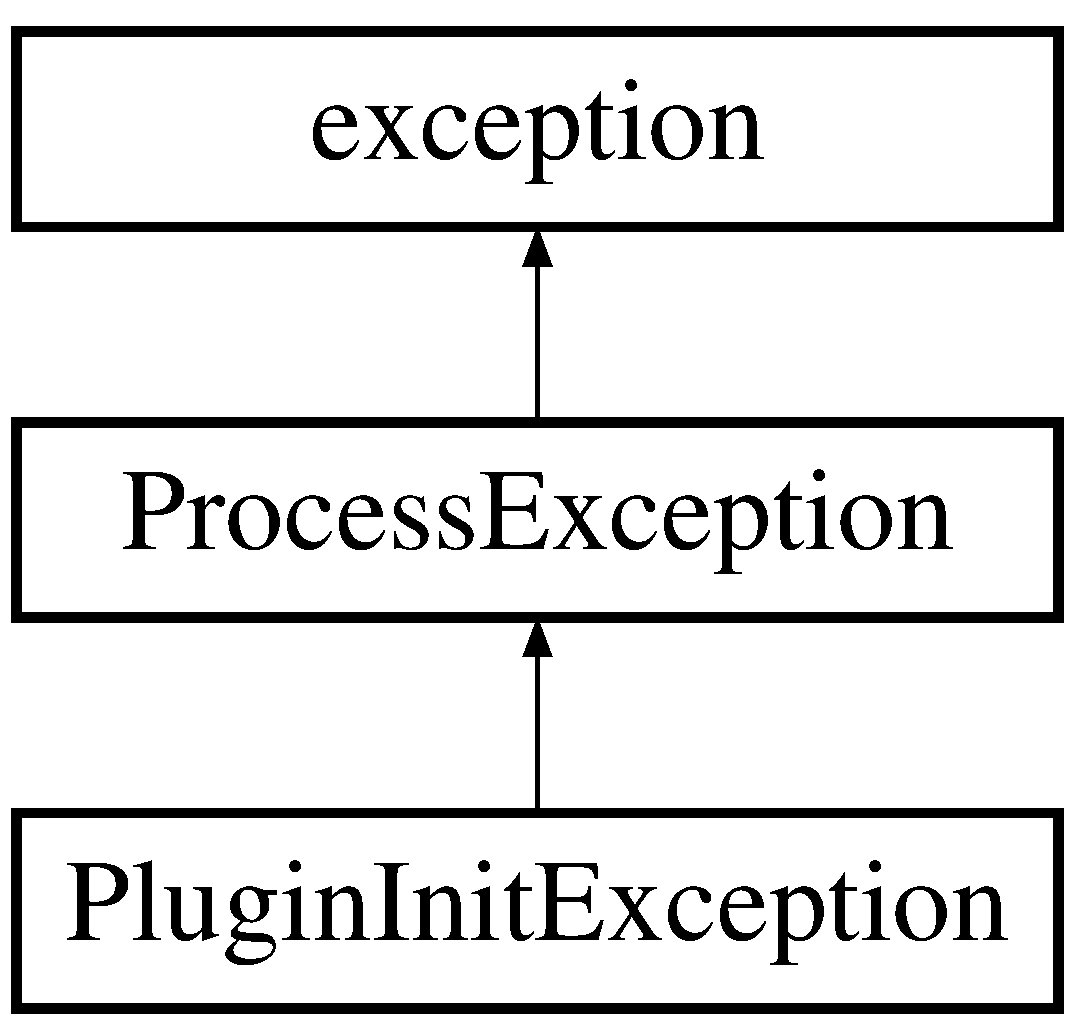
\includegraphics[height=3.000000cm]{class_plugin_init_exception}
\end{center}
\end{figure}
\subsection*{Public Member Functions}
\begin{DoxyCompactItemize}
\item 
\hyperlink{class_plugin_init_exception_a65716fd66b618cdac71d786b186c52c6}{Plugin\+Init\+Exception} (const std\+::string \&msg)
\item 
virtual \hyperlink{class_plugin_init_exception_a2858532ec8c20e597ca43599f11e5933}{$\sim$\+Plugin\+Init\+Exception} () noexcept
\end{DoxyCompactItemize}


\subsection{Detailed Description}


Definition at line 61 of file processexceptions.\+h.



\subsection{Constructor \& Destructor Documentation}
\index{Plugin\+Init\+Exception@{Plugin\+Init\+Exception}!Plugin\+Init\+Exception@{Plugin\+Init\+Exception}}
\index{Plugin\+Init\+Exception@{Plugin\+Init\+Exception}!Plugin\+Init\+Exception@{Plugin\+Init\+Exception}}
\subsubsection[{\texorpdfstring{Plugin\+Init\+Exception(const std\+::string \&msg)}{PluginInitException(const std::string &msg)}}]{\setlength{\rightskip}{0pt plus 5cm}Plugin\+Init\+Exception\+::\+Plugin\+Init\+Exception (
\begin{DoxyParamCaption}
\item[{const std\+::string \&}]{msg}
\end{DoxyParamCaption}
)\hspace{0.3cm}{\ttfamily [inline]}}\hypertarget{class_plugin_init_exception_a65716fd66b618cdac71d786b186c52c6}{}\label{class_plugin_init_exception_a65716fd66b618cdac71d786b186c52c6}


Definition at line 64 of file processexceptions.\+h.

\index{Plugin\+Init\+Exception@{Plugin\+Init\+Exception}!````~Plugin\+Init\+Exception@{$\sim$\+Plugin\+Init\+Exception}}
\index{````~Plugin\+Init\+Exception@{$\sim$\+Plugin\+Init\+Exception}!Plugin\+Init\+Exception@{Plugin\+Init\+Exception}}
\subsubsection[{\texorpdfstring{$\sim$\+Plugin\+Init\+Exception() noexcept}{~PluginInitException() noexcept}}]{\setlength{\rightskip}{0pt plus 5cm}virtual Plugin\+Init\+Exception\+::$\sim$\+Plugin\+Init\+Exception (
\begin{DoxyParamCaption}
{}
\end{DoxyParamCaption}
)\hspace{0.3cm}{\ttfamily [inline]}, {\ttfamily [virtual]}, {\ttfamily [noexcept]}}\hypertarget{class_plugin_init_exception_a2858532ec8c20e597ca43599f11e5933}{}\label{class_plugin_init_exception_a2858532ec8c20e597ca43599f11e5933}


Definition at line 67 of file processexceptions.\+h.



The documentation for this class was generated from the following file\+:\begin{DoxyCompactItemize}
\item 
src/abstractprocess/\hyperlink{processexceptions_8h}{processexceptions.\+h}\end{DoxyCompactItemize}

\hypertarget{class_plugin_load_exception}{}\section{Plugin\+Load\+Exception Class Reference}
\label{class_plugin_load_exception}\index{Plugin\+Load\+Exception@{Plugin\+Load\+Exception}}


{\ttfamily \#include $<$processexceptions.\+h$>$}

Inheritance diagram for Plugin\+Load\+Exception\+:\begin{figure}[H]
\begin{center}
\leavevmode
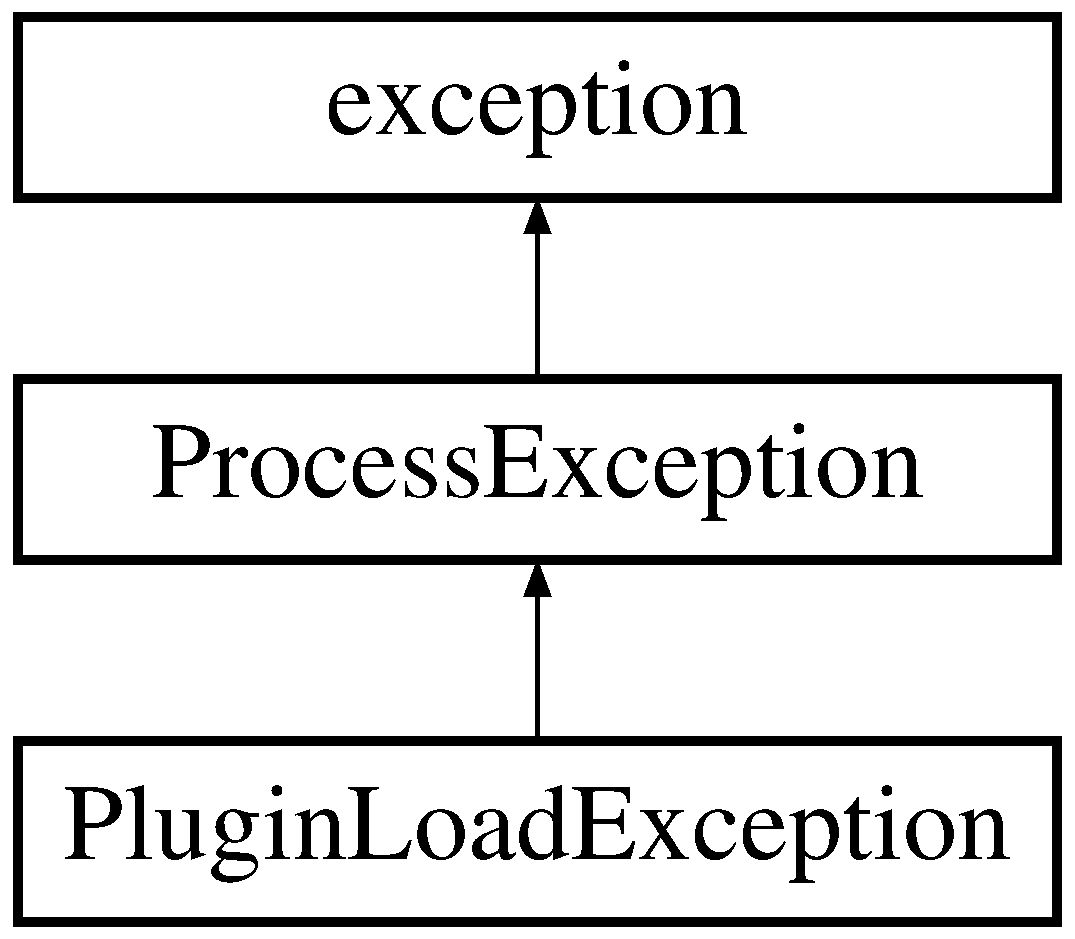
\includegraphics[height=3.000000cm]{class_plugin_load_exception}
\end{center}
\end{figure}
\subsection*{Public Member Functions}
\begin{DoxyCompactItemize}
\item 
\hyperlink{class_plugin_load_exception_a417fcc4d7be702a2caa58fe5e45c784d}{Plugin\+Load\+Exception} (const std\+::string \&msg)
\item 
virtual \hyperlink{class_plugin_load_exception_a81b1e6f7c177e6df99caf2ff384a05f6}{$\sim$\+Plugin\+Load\+Exception} () noexcept
\end{DoxyCompactItemize}


\subsection{Detailed Description}


Definition at line 52 of file processexceptions.\+h.



\subsection{Constructor \& Destructor Documentation}
\index{Plugin\+Load\+Exception@{Plugin\+Load\+Exception}!Plugin\+Load\+Exception@{Plugin\+Load\+Exception}}
\index{Plugin\+Load\+Exception@{Plugin\+Load\+Exception}!Plugin\+Load\+Exception@{Plugin\+Load\+Exception}}
\subsubsection[{\texorpdfstring{Plugin\+Load\+Exception(const std\+::string \&msg)}{PluginLoadException(const std::string &msg)}}]{\setlength{\rightskip}{0pt plus 5cm}Plugin\+Load\+Exception\+::\+Plugin\+Load\+Exception (
\begin{DoxyParamCaption}
\item[{const std\+::string \&}]{msg}
\end{DoxyParamCaption}
)\hspace{0.3cm}{\ttfamily [inline]}}\hypertarget{class_plugin_load_exception_a417fcc4d7be702a2caa58fe5e45c784d}{}\label{class_plugin_load_exception_a417fcc4d7be702a2caa58fe5e45c784d}


Definition at line 55 of file processexceptions.\+h.

\index{Plugin\+Load\+Exception@{Plugin\+Load\+Exception}!````~Plugin\+Load\+Exception@{$\sim$\+Plugin\+Load\+Exception}}
\index{````~Plugin\+Load\+Exception@{$\sim$\+Plugin\+Load\+Exception}!Plugin\+Load\+Exception@{Plugin\+Load\+Exception}}
\subsubsection[{\texorpdfstring{$\sim$\+Plugin\+Load\+Exception() noexcept}{~PluginLoadException() noexcept}}]{\setlength{\rightskip}{0pt plus 5cm}virtual Plugin\+Load\+Exception\+::$\sim$\+Plugin\+Load\+Exception (
\begin{DoxyParamCaption}
{}
\end{DoxyParamCaption}
)\hspace{0.3cm}{\ttfamily [inline]}, {\ttfamily [virtual]}, {\ttfamily [noexcept]}}\hypertarget{class_plugin_load_exception_a81b1e6f7c177e6df99caf2ff384a05f6}{}\label{class_plugin_load_exception_a81b1e6f7c177e6df99caf2ff384a05f6}


Definition at line 58 of file processexceptions.\+h.



The documentation for this class was generated from the following file\+:\begin{DoxyCompactItemize}
\item 
src/abstractprocess/\hyperlink{processexceptions_8h}{processexceptions.\+h}\end{DoxyCompactItemize}

\hypertarget{class_process_exception}{}\section{Process\+Exception Class Reference}
\label{class_process_exception}\index{Process\+Exception@{Process\+Exception}}


{\ttfamily \#include $<$processexceptions.\+h$>$}

Inheritance diagram for Process\+Exception\+:\begin{figure}[H]
\begin{center}
\leavevmode
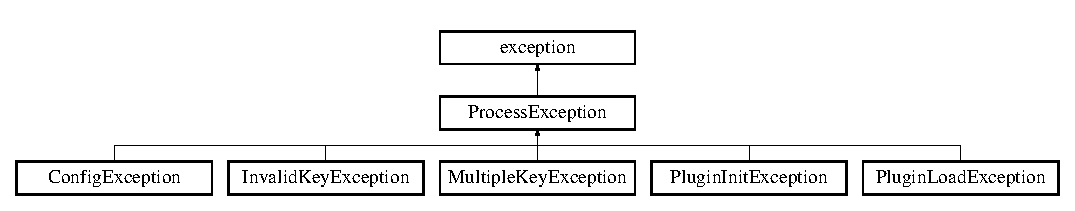
\includegraphics[height=2.382979cm]{class_process_exception}
\end{center}
\end{figure}
\subsection*{Public Member Functions}
\begin{DoxyCompactItemize}
\item 
\hyperlink{class_process_exception_a1f5b03237ffd6f7d3266366d8183a3d2}{Process\+Exception} (const std\+::string \&msg)
\item 
virtual \hyperlink{class_process_exception_aaa12fd4e0772f0fcc45946f9df629393}{$\sim$\+Process\+Exception} () noexcept
\item 
const char $\ast$ \hyperlink{class_process_exception_a801d552880578f3ad6848c241ec3d7bc}{what} () const  noexcept
\end{DoxyCompactItemize}


\subsection{Detailed Description}


Definition at line 6 of file processexceptions.\+h.



\subsection{Constructor \& Destructor Documentation}
\index{Process\+Exception@{Process\+Exception}!Process\+Exception@{Process\+Exception}}
\index{Process\+Exception@{Process\+Exception}!Process\+Exception@{Process\+Exception}}
\subsubsection[{\texorpdfstring{Process\+Exception(const std\+::string \&msg)}{ProcessException(const std::string &msg)}}]{\setlength{\rightskip}{0pt plus 5cm}Process\+Exception\+::\+Process\+Exception (
\begin{DoxyParamCaption}
\item[{const std\+::string \&}]{msg}
\end{DoxyParamCaption}
)\hspace{0.3cm}{\ttfamily [inline]}}\hypertarget{class_process_exception_a1f5b03237ffd6f7d3266366d8183a3d2}{}\label{class_process_exception_a1f5b03237ffd6f7d3266366d8183a3d2}


Definition at line 9 of file processexceptions.\+h.

\index{Process\+Exception@{Process\+Exception}!````~Process\+Exception@{$\sim$\+Process\+Exception}}
\index{````~Process\+Exception@{$\sim$\+Process\+Exception}!Process\+Exception@{Process\+Exception}}
\subsubsection[{\texorpdfstring{$\sim$\+Process\+Exception() noexcept}{~ProcessException() noexcept}}]{\setlength{\rightskip}{0pt plus 5cm}virtual Process\+Exception\+::$\sim$\+Process\+Exception (
\begin{DoxyParamCaption}
{}
\end{DoxyParamCaption}
)\hspace{0.3cm}{\ttfamily [inline]}, {\ttfamily [virtual]}, {\ttfamily [noexcept]}}\hypertarget{class_process_exception_aaa12fd4e0772f0fcc45946f9df629393}{}\label{class_process_exception_aaa12fd4e0772f0fcc45946f9df629393}


Definition at line 13 of file processexceptions.\+h.



\subsection{Member Function Documentation}
\index{Process\+Exception@{Process\+Exception}!what@{what}}
\index{what@{what}!Process\+Exception@{Process\+Exception}}
\subsubsection[{\texorpdfstring{what() const  noexcept}{what() const  noexcept}}]{\setlength{\rightskip}{0pt plus 5cm}const char$\ast$ Process\+Exception\+::what (
\begin{DoxyParamCaption}
{}
\end{DoxyParamCaption}
) const\hspace{0.3cm}{\ttfamily [inline]}, {\ttfamily [noexcept]}}\hypertarget{class_process_exception_a801d552880578f3ad6848c241ec3d7bc}{}\label{class_process_exception_a801d552880578f3ad6848c241ec3d7bc}


Definition at line 15 of file processexceptions.\+h.



The documentation for this class was generated from the following file\+:\begin{DoxyCompactItemize}
\item 
src/abstractprocess/\hyperlink{processexceptions_8h}{processexceptions.\+h}\end{DoxyCompactItemize}

\chapter{File Documentation}
\hypertarget{abstractprocess_8cpp}{}\section{src/abstractprocess/abstractprocess.cpp File Reference}
\label{abstractprocess_8cpp}\index{src/abstractprocess/abstractprocess.\+cpp@{src/abstractprocess/abstractprocess.\+cpp}}
{\ttfamily \#include \char`\"{}abstractprocess.\+h\char`\"{}}\\*
{\ttfamily \#include \char`\"{}coreclient.\+h\char`\"{}}\\*
{\ttfamily \#include \char`\"{}xmlconfigurationreader.\+h\char`\"{}}\\*
{\ttfamily \#include \char`\"{}processconfiguration.\+h\char`\"{}}\\*
{\ttfamily \#include \char`\"{}getopt.\+h\char`\"{}}\\*
{\ttfamily \#include \char`\"{}configurationpluginparameter.\+h\char`\"{}}\\*
{\ttfamily \#include \char`\"{}plugininterface.\+h\char`\"{}}\\*
{\ttfamily \#include $<$Q\+Core\+Application$>$}\\*
{\ttfamily \#include $<$Qt\+Gui/\+Q\+Application$>$}\\*

\hypertarget{abstractprocess_8h}{}\section{src/abstractprocess/abstractprocess.h File Reference}
\label{abstractprocess_8h}\index{src/abstractprocess/abstractprocess.\+h@{src/abstractprocess/abstractprocess.\+h}}
{\ttfamily \#include $<$Q\+Object$>$}\\*
{\ttfamily \#include $<$Q\+Hash$>$}\\*
{\ttfamily \#include $<$memory$>$}\\*
{\ttfamily \#include \char`\"{}processexceptions.\+h\char`\"{}}\\*
{\ttfamily \#include \char`\"{}common.\+h\char`\"{}}\\*
\subsection*{Classes}
\begin{DoxyCompactItemize}
\item 
class \hyperlink{class_abstract_process}{Abstract\+Process}
\begin{DoxyCompactList}\small\item\em The \hyperlink{class_abstract_process}{Abstract\+Process} class  Класс процеса, расширяемого плагинами \end{DoxyCompactList}\end{DoxyCompactItemize}

\hypertarget{main_8cpp}{}\section{src/abstractprocess/main.cpp File Reference}
\label{main_8cpp}\index{src/abstractprocess/main.\+cpp@{src/abstractprocess/main.\+cpp}}
{\ttfamily \#include $<$Q\+Debug$>$}\\*
{\ttfamily \#include $<$stdexcept$>$}\\*
{\ttfamily \#include \char`\"{}cleanexit.\+h\char`\"{}}\\*
{\ttfamily \#include \char`\"{}abstractprocess.\+h\char`\"{}}\\*
\subsection*{Functions}
\begin{DoxyCompactItemize}
\item 
int \hyperlink{main_8cpp_a0ddf1224851353fc92bfbff6f499fa97}{main} (int argc, char $\ast$argv\mbox{[}$\,$\mbox{]})
\end{DoxyCompactItemize}
\subsection*{Variables}
\begin{DoxyCompactItemize}
\item 
const char $\ast$ \hyperlink{main_8cpp_adc0221a311d122f5c20b9ce7982f95ee}{optstr} = \char`\"{}n\+:s\+:c\+:\char`\"{}
\end{DoxyCompactItemize}


\subsection{Function Documentation}
\index{main.\+cpp@{main.\+cpp}!main@{main}}
\index{main@{main}!main.\+cpp@{main.\+cpp}}
\subsubsection[{\texorpdfstring{main(int argc, char $\ast$argv[])}{main(int argc, char *argv[])}}]{\setlength{\rightskip}{0pt plus 5cm}int main (
\begin{DoxyParamCaption}
\item[{int}]{argc, }
\item[{char $\ast$}]{argv\mbox{[}$\,$\mbox{]}}
\end{DoxyParamCaption}
)}\hypertarget{main_8cpp_a0ddf1224851353fc92bfbff6f499fa97}{}\label{main_8cpp_a0ddf1224851353fc92bfbff6f499fa97}


Definition at line 8 of file main.\+cpp.



\subsection{Variable Documentation}
\index{main.\+cpp@{main.\+cpp}!optstr@{optstr}}
\index{optstr@{optstr}!main.\+cpp@{main.\+cpp}}
\subsubsection[{\texorpdfstring{optstr}{optstr}}]{\setlength{\rightskip}{0pt plus 5cm}const char$\ast$ optstr = \char`\"{}n\+:s\+:c\+:\char`\"{}}\hypertarget{main_8cpp_adc0221a311d122f5c20b9ce7982f95ee}{}\label{main_8cpp_adc0221a311d122f5c20b9ce7982f95ee}


Definition at line 6 of file main.\+cpp.


\hypertarget{processexceptions_8h}{}\section{src/abstractprocess/processexceptions.h File Reference}
\label{processexceptions_8h}\index{src/abstractprocess/processexceptions.\+h@{src/abstractprocess/processexceptions.\+h}}
{\ttfamily \#include $<$stdexcept$>$}\\*
\subsection*{Classes}
\begin{DoxyCompactItemize}
\item 
class \hyperlink{class_process_exception}{Process\+Exception}
\item 
class \hyperlink{class_invalid_key_exception}{Invalid\+Key\+Exception}
\item 
class \hyperlink{class_multiple_key_exception}{Multiple\+Key\+Exception}
\item 
class \hyperlink{class_config_exception}{Config\+Exception}
\item 
class \hyperlink{class_plugin_load_exception}{Plugin\+Load\+Exception}
\item 
class \hyperlink{class_plugin_init_exception}{Plugin\+Init\+Exception}
\end{DoxyCompactItemize}

%--- End generated contents ---

% Index
\backmatter
\newpage
\phantomsection
\clearemptydoublepage
\addcontentsline{toc}{chapter}{Index}
\printindex

\end{document}
